\subsubsection{Mémoire distribuée}
En mémoire distribuée, nous n'effectuons pas les mêmes calculs qu'en mémoire partagée, mais les accélérations obtenues nous donnerons une approximation des performances que nous pourrons obtenir.
%
Sur la machine Rostand, la factorisation atteint une accélération de 11,8 et la résolution triangulaire une accélération de 3,5.
%
Sur la machine Manumanu, cette accélération monte à 93 pour la factorisation (Fig.~\ref{fig:res_facto_mpi_manu}) et à 73 pour la résolution triangulaire (Fig.~\ref{fig:res_trsv_mpi_manu}).


%   (-_-)   %
\begin{figure}[!h]
     \begin{center}
        \subfigure[Factorisation ILU(0).]{
          \label{fig:res_facto_mpi_manumanu}
          \includegraphics[width=0.48\textwidth]{res_facto_mpi_manu}
        }
        \subfigure[Résolution triangulaire]{
          \label{fig:res_trsv_mpi_manumanu}
          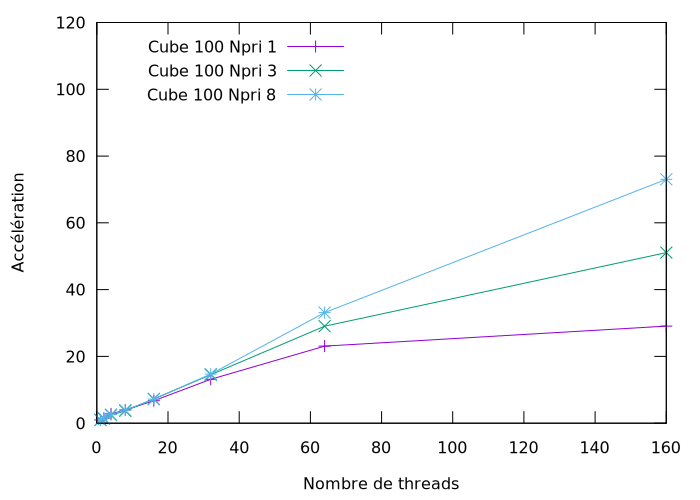
\includegraphics[width=0.48\textwidth]{res_trsv_mpi_manu}
        }
    \end{center}
    \caption{Performances sur Manumanu en mémoire distribuée.}
\end{figure}
